\documentclass[10pt]{beamer}
\usepackage[utf8]{inputenc}
\usepackage{tikz}
\usetikzlibrary{automata, positioning}
\usepackage{hyperref}

\usepackage[absolute,overlay]{textpos}
\usepackage{graphicx}
\usepackage{listings}
\lstset{
  language=Python,
  basicstyle=\ttfamily\scriptsize,
  commentstyle=\color{gray},
  keywordstyle=\color{blue},
  stringstyle=\color{red},
  showstringspaces=false,
  numbers=left,
  numberstyle=\tiny,
  frame=single,
  breaklines=true,
}

\mode<presentation> {
\usetheme{boxes} % When headline is wanted use Dresden theme instead
\usecolortheme{seagull}
\logo{\includegraphics[height=1.5cm]{ku_logo_dk}}
\setbeamertemplate{footline}[frame number]
% \setbeamertemplate{footline}{
%   \hspace{1em}
%   \hfill
%   \insertframenumber/\inserttotalframenumber
%   \vspace{1em}
%   \hspace{1em}
%   \includegraphics[height=2cm]{ku_logo_dk}
%   \hspace{1em}
% }
\setbeamertemplate{navigation symbols}{}
\setbeamertemplate{itemize items}[square]
}


%----------------------------------------------------------------------------------------
%	TITLE PAGE
%----------------------------------------------------------------------------------------

\title[Kickstart-kursus] % bottom of every slide
  {Kickstart-kursus i programmering 23 dag 4\\ Finite States} %\includegraphics[height=5cm]{images/gozz}} % title page



\author{\footnotesize{Daniel Spikol} \\
          \footnotesize{\texttt{ds@di.ku.dk}}}

\institute {DIKU \\ Københavns Universitet}

\date[17. august 2023]{17 august 2023}

\begin{document}
\begin{frame}[plain]
\titlepage
\end{frame}
%%----------------------------------------------%%
\begin{frame}{Recap from Wednesday}
   	\begin{itemize}
	\item Scoping
	\item Conditionals
	\item Projects
	\end{itemize}
\end{frame}

%%----------------------------------------------%%

\begin{frame}{Thursday IFOs}
  \begin{itemize}
  \item Finite State Machines
   \item Wrapping up Things
  \item Projects and Demos
  \end{itemize}
\end{frame}

%%----------------------------------------------%%

\begin{frame}{Finite State Machines- FSM}
A Finite State Machine (FSM) is a mathematical model of computation used to design algorithms.
In the context of computer games, FSMs are often used for character behaviour, where different states might represent actions like ``dle", ``attack", ``defend", or ``flee", and game events or conditions determine transitions between states.

\end{frame}

%%----------------------------------------------%%

\begin{frame}{The STATES in a FSM}
	\begin{itemize}
	\item \textbf{Discrete States:} An FSM consists of a limited or finite number of states. It can be in just one of these states at any given moment. Transitions define how it changes from one state to another based on inputs or conditions.
	\item \textbf{Transitions \& Triggers:} Events or conditions trigger transitions between states. Each state specifies which state the machine will move to next for each possible input.
	\item \textbf{Start and End States:} Among the finite states, there is one initial state where the FSM begins its operation. Additionally, there can be one or more end states where the FSM is considered to be completed or final.
	\end{itemize}
\end{frame}


%%----------------------------------------------%%

\begin{frame}{The Classic Example}
  
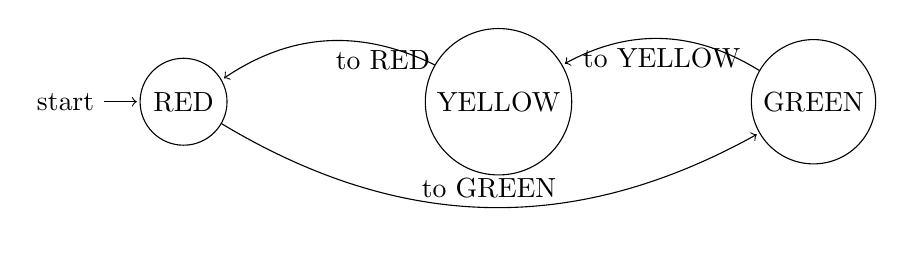
\begin{tikzpicture}[shorten >=1pt, node distance=4cm, on grid, auto]
    \node[state, initial] (R)   {RED};
    \node[state] (Y) [right=of R] {YELLOW};
    \node[state] (G) [right=of Y] {GREEN};
    
    \path[->]
    (R) edge[bend right] node {to GREEN} (G)
    (G) edge[bend right] node {to YELLOW} (Y)
    (Y) edge[bend right] node {to RED} (R);
\end{tikzpicture}	

\end{frame}


%%----------------------------------------------%%
\begin{frame}{Mathematical Abstraction of the FSM}
\begin{itemize}
\item A finite state machine is a mathematical abstraction used to design algorithms. In simple terms, a state machine will read a series of inputs.
\item When it reads an input, it will switch to a different state. Each state specifies which state to switch to for a given input.
\end{itemize}
\end{frame}

%%----------------------------------------------%%
\begin{frame}{IDEAL Problem Solving}
\begin{center}
    	 \includegraphics[height=7cm]{images/traffic}
\end{center}
\end{frame}

%%----------------------------------------------%%
\begin{frame}[fragile]{Code FSM}
\begin{lstlisting}
# States for our FSM
STATE_RED = "RED"
STATE_GREEN = "GREEN"

# Initial state
current_state = STATE_RED

def setup():
    size(200, 200)
    fill(255)

def draw():
    background(200)
    
    if current_state == STATE_RED:
        fill(255, 0, 0)  # Red color for RED state
    elif current_state == STATE_GREEN:
        fill(0, 255, 0)  # Green color for GREEN state
    
    ellipse(width/2, height/2, 100, 100)

def mousePressed():
    global current_state
    if current_state == STATE_RED:
        current_state = STATE_GREEN
    elif current_state == STATE_GREEN:
        current_state = STATE_RED
\end{lstlisting}
\end{frame}

%%----------------------------------------------%%

\begin{frame}{We Code a bit}{We make a Traffic Light}

\begin{itemize}
	 \item How do we add the Yellow?
	 \item Let's do it together...
\end{itemize}
\end{frame}



%%----------------------------------------------%%

\begin{frame}{Game States}
\begin{center}
    	 \includegraphics[height=7cm]{images/gameflowchart}
\end{center}
\end{frame}

%%----------------------------------------------%%

\begin{frame}{IDEAL Problem Solving}
\begin{center}
    	 \includegraphics[height=6cm]{images/superm}
\end{center}
\end{frame}

%%----------------------------------------------%%
\begin{frame}{IDEAL Problem Solving}
\begin{center}
    	 \includegraphics[height=7cm]{images/mariobig}
\end{center}
\end{frame}

%%----------------------------------------------%%

\begin{frame}{Game States}
\begin{center}
    	 \includegraphics[height=7cm]{images/gameflowchart}
\end{center}
\end{frame}

%%----------------------------------------------%%

\begin{frame}{Diagram It}

\begin{center}
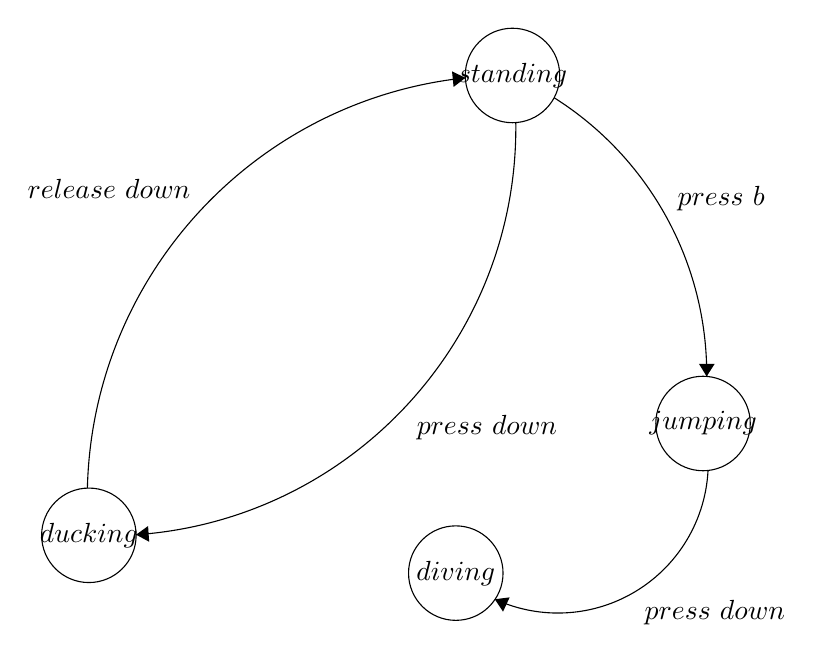
\begin{tikzpicture}[scale=0.2]
\tikzstyle{every node}+=[inner sep=0pt]
\draw [black] (38.1,-9.3) circle (3);
\draw (38.1,-9.3) node {$standing$};
\draw [black] (34.5,-40.9) circle (3);
\draw (34.5,-40.9) node {$diving$};
\draw [black] (50.2,-31.4) circle (3);
\draw (50.2,-31.4) node {$jumping$};
\draw [black] (11.2,-38.5) circle (3);
\draw (11.2,-38.5) node {$ducking$};
\draw [black] (11.106,-35.503) arc (-181.39782:-263.90676:26.859);
\fill [black] (35.11,-9.45) -- (34.26,-9.04) -- (34.36,-10.03);
\draw (17.67,-16.5) node [left] {$release\mbox{ }down$};
\draw [black] (40.744,-10.712) arc (57.75845:-0.35604:20.774);
\fill [black] (50.43,-28.41) -- (50.94,-27.61) -- (49.94,-27.61);
\draw (48.55,-17.12) node [right] {$press\mbox{ }b$};
\draw [black] (38.31,-12.291) arc (0.70861:-86.01319:25.916);
\fill [black] (14.2,-38.46) -- (15.03,-38.91) -- (14.96,-37.91);
\draw (31.99,-31.63) node [right] {$press\mbox{ }down$};
\draw [black] (50.518,-34.371) arc (-2.8958:-114.7483:9.548);
\fill [black] (36.98,-42.56) -- (37.5,-43.35) -- (37.92,-42.44);
\draw (50.95,-42.56) node [below] {$press\mbox{ }down$};
\end{tikzpicture}
\end{center}
\end{frame}

%%----------------------------------------------%%

\begin{frame}{Let's make some FSM diagrams}
   	\href {https://markusfeng.com/projects/graph/}https://markusfeng.com/projects/graph/
\end{frame}

%%----------------------------------------------%%
\begin{frame}{Today' Recap}
   	\begin{itemize}
	\item Conditionals
	\item FSM
	\item Projects
	\end{itemize}
\end{frame}

%%----------------------------------------------%%

\begin{frame}{Tomorrow}
   	\begin{itemize}
	\item Morning code
	\item Afternoon Show and Talk
	\end{itemize}
\end{frame}
%%----------------------------------------------%%
%%----------------------------------------------%%
%%----------------------------------------------%%
\end{document}